\documentclass{beamer}
\usepackage[T1]{fontenc}
\usepackage[utf8]{inputenc}
\usepackage[dvipdfm]{graphicx}
\usepackage{graphics,latexsym}
\usepackage{graphicx}
\usepackage{amsmath}
\usepackage{natbib}
\usepackage[dvips]{color}
\usepackage{subfigure}
\usepackage{verbatim}
\usetheme{Warsaw}
\usecolortheme{default}
\useoutertheme{shadow}
\useinnertheme{rectangles}

\bibpunct{(}{)}{;}{a}{,}{,}

\title[Inference in HBNs]{Inference in Hybrid Bayesian Networks}
\subtitle{state-of-the-art}
\author[Carlos Badenes]{{Carlos Badenes}\\
{\small Computational Intelligence Group, Departamento de Inteligencia Artificial, Universidad Polit\'ecnica de Madrid, Spain}}
\date{}

\begin{document}

\frame{\titlepage}

\begin{frame}
	 \frametitle{Hybrid Bayesian Networks}
	\begin{itemize}
  	  \item Hybrid models are used for representing uncertainty in domains containing not only discrete variables, but also continuous values such as distance, temperature or location.

  	  \item The introduction of continuous variables in a graphical model has several particularities: factors that imply continuous variables and marginalization

	  \item The complexity of these algorithms is so high that present significant challenges to perfom
  	\end{itemize}
\end{frame}

\begin{frame}
	   \frametitle{Hybrid Bayesian Networks}
	\begin{itemize}
  	  \item Heskes and Zoeter (2003) applied a generalized belief propagation to approximate inference in HBNs\[
mean: E[x], covariance: E[(x-E[x])(y-E[y])]
\]	
  	  \item Schrempf and Hanebeck, 2004 considered that using  first two moments is a drawback
  	\end{itemize} 
\end{frame}

\begin{frame}
	   \frametitle{Hybrid Bayesian Networks}
		\begin{figure}
		  	\centering
    			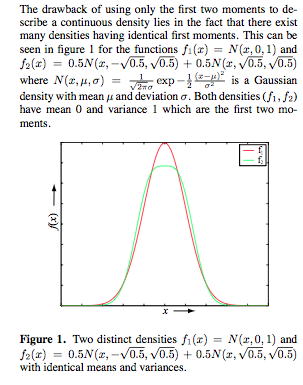
\includegraphics[width=0.7\textwidth]{HBM-2004.png}
  			\caption{Drawback}
		\end{figure}
\end{frame}

\begin{frame}
	\frametitle{Hybrid Bayesian Networks}
	Barry R. Cobb and Prakash P. Shenoy proposed alternatives to discretizacion for solving HBNs.

	\begin{itemize}
		\item 2004: Deterministic variables with \textit{Conditional Linear Gaussian (CLG)} 

		\item 2005: Continuous variables not normally distributed with \textit{Mixtures of Truncated Exponentials (MTE)} potentials

		\item 2006: Discrete and continuous variables with \textit{Mixture of Gaussians (MoG)} BNs
	\end{itemize}
\end{frame}

\begin{frame}
	\frametitle{Hybrid Bayesian Networks}
	In a general HBN with nonlinear and/or non Gaussian variables there is no existing method that could produce exact posterior distribution.

	\begin{itemize}
		\item \textit{Hybrid Loopy Belief Propagation(HLBP)}

		\item \textit{Loopy Belief Propagation(LBP)}

		\item \textit{Nonparametric Belief Propagation(NBP)}
	\end{itemize}
\end{frame}

\begin{frame}
	\frametitle{Hybrid Bayesian Networks}
	Sun et al., 2010 describe an algorithm able to provide an exact solution for polytree networks, and approximate solution by loopy propagation for general hybrid models. 
	\begin{itemize}
		\item \textit{Direct Message Passing for Hybrid Bayesian Network} (DMP-HBN)
	\end{itemize}
\end{frame}

\begin{frame}
	\frametitle{Conclusions and future research}
In this short state-of-the-art we have reviewed some of the most important research papers on inference in Hybrid Bayesian Networks published to date and the algorithms proposed to resolve it.

The quality of these algorithms, quality as the performance and accuracy, is constantly evolving and improving. Being this aspect the main line of research actually.
\end{frame}

\end{document}